\begin{exercice*}[Pavage bis]
    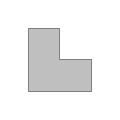
\begin{tikzpicture}[scale=0.4]            
        % \draw[help lines, color=black!30] (0,0) grid (16,16);            
        \begin{scope}[shift={(0,16)},rotate around={90:(16,0)}]
            \coordinate (O) at (16,0);
            \tkzDrawPoints[shape=cross out,size=3pt](O);
            \tkzLabelPoints[above](O);
            \pavageL
            \begin{scope}[shift={(-8,8)}]
                \pavageL
            \end{scope}
            \begin{scope}[rotate around={90:(8,0)}]
                \pavageL
            \end{scope}
            \begin{scope}[rotate around={-90:(16,8)}]
                \pavageL
            \end{scope}
        \end{scope}
        % Les points
        \coordinate (A) at (12,12);
        \coordinate (B) at (14,12);
        \coordinate (C) at (14,13);
        \coordinate (D) at (13,13);
        \coordinate (E) at (13,14);
        \coordinate (F) at (12,14);
        \draw[color=gray,fill=gray,fill opacity=0.5] (A) -- (B) -- (C) -- (D) -- (E) -- (F) -- cycle;        
    \end{tikzpicture}
    \begin{enumerate}
        \item Colorier \textbf{en bleu} l'image de la figure grise 
        
        par l'homothétie de centre $O$ et de rapport $2$.
        \item Colorier \textbf{en rouge} l'image de la figure grise 
        
        par l'homothétie de centre $O$ et de rapport $4$.        
    \end{enumerate}

\end{exercice*}
\begin{corrige}
    %\setcounter{partie}{0} % Pour s'assurer que le compteur de \partie est à zéro dans les corrigés
    \phantom{rrr}

    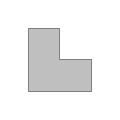
\begin{tikzpicture}[scale=0.4]            
        % \draw[help lines, color=black!30] (0,0) grid (16,16);            
        \begin{scope}[shift={(0,16)},rotate around={90:(16,0)}]
            \coordinate (O) at (16,0);
            \tkzDrawPoints[shape=cross out,size=3pt](O);
            \tkzLabelPoints[above](O);
            \pavageL
            \begin{scope}[shift={(-8,8)}]
                \pavageL
            \end{scope}
            \begin{scope}[rotate around={90:(8,0)}]
                \pavageL
            \end{scope}
            \begin{scope}[rotate around={-90:(16,8)}]
                \pavageL
            \end{scope}
        \end{scope}
        % Les points
        \coordinate (A) at (12,12);
        \coordinate (B) at (14,12);
        \coordinate (C) at (14,13);
        \coordinate (D) at (13,13);
        \coordinate (E) at (13,14);
        \coordinate (F) at (12,14);
        \draw[color=gray,fill=gray,fill opacity=0.5] (A) -- (B) -- (C) -- (D) -- (E) -- (F) -- cycle;
        \imageHomothetyHexaGone{2}{blue};
        \imageHomothetyHexaGone{4}{red};
    \end{tikzpicture}

    \begin{enumerate}
        \item Colorier \textbf{en bleu} l'image de la figure grise par l'homothétie de centre $O$ et de rapport $2$.
        \item Colorier \textbf{en rouge} l'image de la figure grise par l'homothétie de centre $O$ et de rapport $4$.        
    \end{enumerate}
\end{corrige}

